\subsection{From augmented posets to decorated posets and back}
\label{sec:abstract_decoration}

\begin{definition}[Abstractions]
  From a causal trace $\theta$ define an \emph{abstraction} function $\mathsf{decoration\_of\_trace}$ that maps a trace into a decorated poset as follows:
  \begin{align*}
    &\mathsf{decoration\_of\_trace}(t_i:M_i\overset{m,p}{\Rightarrow} M_{i+1}) = e_i \\
    &e_i \redl{+}_s e_j \iff t_i <_{\theta}^s t_j, \labl(t_i)\redl{+}_s \labl(t_j)\\
    &e_i \redl{-}_s e_j \iff t_i \dashv_{\theta} t_j, \labl(t_i) \redl{-}_s \labl(t_j).
  \end{align*}
  From an decorated poset $(E,\redl{+},\redl{-},\labl)$ define the abstraction $\alpha'$ that returns the augmented poset $(E,\cover,\prec,\dashv,\labl)$ defined as follows:
  \begin{align*}
    &e\prec e'\iff e\redl{+}_s e'\\
    &e\cover e'\iff e\redl{+}_s e'\text{ and }\nexists e''\text{ s.t. }e\redl{+}_s e'', e''\redl{+}_s e'\\
    &e\dashv e'\iff e\redl{-}_s e'.
  \end{align*}
\end{definition}

In the following chain of abstractions:
  \[
  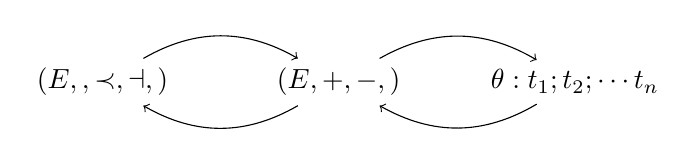
\begin{tikzpicture} %[scale=0.8]
%    \node (s) at (0,0) {\((E,\leq,\labl)\)};
    \node (as) at (3,0) {\((E,\cover,\prec,\dashv,\labl)\)};
    \node (ds) at (6,0) {\((E,\redl{+},\redl{-},\labl)\)};
    \node (trace) at (9,0) {\(\theta:t_1;t_2;\cdots t_n\)};
%    \draw [->] (s) to [bend left] (as);
%    \draw [->] (as) to [bend left] (s);
    \draw [->] (ds) to [bend left] (as);
    \draw [->] (as) to [bend left] (ds);
    \draw [->] (ds) to [bend left] (trace);
    \draw [->] (trace) to [bend left] (ds);
  \end{tikzpicture}
  \]
the definition above covers the abstractions from causal traces to decorated posets and from decorated posets to augmented posets. The abstractio of~\autoref{def:abstraction} is the composition of the two. The concretisation function from an augmented poset to a decorated one returns all decorations of~\autoref{def:decorate_poset} that are valid.
